\documentclass{article}
\usepackage{graphicx} % Required for inserting images
\usepackage{natbib}
\usepackage{amsmath}
\usepackage{comment}
\usepackage{url} 
\usepackage[hidelinks]{hyperref}
\usepackage[T1]{fontenc}
\usepackage{mathpazo,euler}
\usepackage[scaled=0.9]{DejaVuSans}
\usepackage[utf8]{inputenc}
\usepackage{listings}
\usepackage{tabularx}
\usepackage{amsfonts}
\usepackage{booktabs}
\usepackage{siunitx}
\usepackage{geometry}
\usepackage[font=tiny,labelfont=bf]{caption}
\usepackage{float} % At the beginning of your document

\geometry{margin=1.5in}
\lstset{basicstyle=\ttfamily}
%\documentclass[11pt]{article}
\setlength{\parskip}{1em} % 1em is an example value; adjust as needed
\bibliographystyle{abbrvnat}
\setcitestyle{authoryear,open={(},close={)}} % Citation-related commands

%\title{First Year Paper}
\title{Genetic Architecture Implications on Rapid Evolutionary Dynamics} % Add your subtitle here
% title ideas
% Genetic architecture implication on rapid evolutionary dynamics & detectability of causal loci after a rapid evolution event  



%\subtitle(Advisor: Moisés Expósito Alonso)
\author{Tatiana Bellagio \\ Advisor: Moisés Expósito Alonso}
\date{November 2023}

\let\oldparagraph\paragraph
\renewcommand{\paragraph}[1]{\oldparagraph{#1}\mbox{}\\}

\begin{document}

\maketitle

\begin{abstract}
In the face of anthropogenic climate and land use crises, environments are changing faster than ever and species must adapt to keep up and avoid extinction. While this has motivated much theoretical and simulation-based research to study the role of genetic architecture in rapid environmental adaptation, these studies are rarely parameterized with realistic setups let alone validated through feasible experiments. Here, I use population genetic simulations varying genetic architecture parameters, from monogenic to polygenic, from low heritable to high heritable traits, coded by low to high frequency alleles, in experimental setups that closely match an experimental evolution design with \textit{Arabidopsis thaliana}. These include realistic population sizes, survival and fecundity distributions, partial selfing, strengths of selection, and starting genetic material through simulations with whole-genome variant data. I then investigate the effect of such parameters and the outcome of population adaptation or extinction. My results indicate that traits with higher polygenicity significantly enhance survival probabilities in rapidly changing environments, while the influence of heritability, contrary to common intuition, is context dependent with positive or negative influence depending on genetic architecture complexity.
\end{abstract}

\tableofcontents
\newpage % Starts a new page after the table of contents

\section{Introduction}
\subsection{Shift, Adapt or Perish}
When species face environmental changes that displace them from their ecological niche, there are only three possible outcomes: shift their geographical distribution to track suitable environments, adapt to the newly imposed conditions, or face local to global extinction. Adaptation is the process by which a population becomes better suited to the new environment through natural selection acting over the population's standing and de novo genetic variation. In the face of rapid anthropogenic  environmental changes \citep{IPCC2023}, adaptation through evolution must also be rapid to ensure persistence of populations and avoid extinction. Thus, specifically understanding rapid eco-evolutionary dynamics and outcomes has become of utmost importance \citep{Waldvogel2020-dh, Palumbi2002-li, Stockwell2003-da}. 

\subsection{What is rapid evolution?}
Evolution has been historically thought of as a slow and gradual process occurring over extensive timescales, often spanning thousands to millions of years. However, genetically based rapid phenotypic changes have been shown to be pervasive in nature, such as the famous peppered moth \citep{Cook2013-bs}, insecticide resistance in \textit{Drosophila} \citep{Daborn2002-is},  beak size in Darwin’s finches \citep{Grant2008-uc}, \textit{Brassica rapa} flowering time in response to climate fluctuations \citep{Franks2007-ys}, and the evolved resistance to agricultural products in more than 200 plant species \citep{Heap2020}. 

Rapid evolution, can be defined based on the short number of generations in which a genetic change occurs, but also as the convergence of ecological and evolutionary times \citep{Hairston2005-qo}. This highlights the importance of rapid evolution as one of the more applied domains within evolutionary biology. Coupled with advances in genome sequencing technology that have led to an increase in the genomic data on non-model organisms, the understanding of eco-evolutionary dynamics have the potential to address urgent conservation issues. Understanding and predicting the pace and direction of evolutionary changes can inform conservation strategies and management practices. \citep{Bay2017-uu, Coulson2017-yh, Forester2022-yl}.

As highlighted in \citep{Yamamichi2022-yj} short-term eco-evolutionary dynamics, despite their inherent interdisciplinary nature, have been mostly studied solely from an ecological perspective and tend to focus on adaptation at the phenotypic level without considering the genetic part of the evolutionary process. More studies are needed in the evolutionary aspect of rapid adaptation to understand intertwined processes and to make more accurate predictions. \citep{Rudman2022-uc}

\subsection{Trait architecture and its potential impact in adaptation}
Discussions concerning  how and where adaptive loci are distribute across the genome have come a long way. Since Darwin \citep{Darwin1859-yh} and Huxley \citep{Huxley1860} there has been debates about whether the nature of adaptation is characterized by incremental, subtle variations in many loci or by abrupt changes on only a few of them. These are foundational unsolved questions in evolutionary biology, with compelling evidence showing that both cases can be true, and that there is considerable heterogeneity in architectures among adaptive traits \citep{Orr1992-xj, Orr1998-pr}, let alone complexities not discussed here including  the effect of structural variation, epistasis, pleiotropy, and ploidy. 

The implications of genetic architecture on population dynamics have been widely documented. For example, genetic architecture acting as a buffer for adaptive alleles through dominance \citep{Yamamichi2017-uj}, or the implication of the number of loci affecting reproductive incompatibility and determining speciation \citep{Orr1996-eq}. Many more are listed in \citep{Bertram2019-sg}. Delving deeper on a more narrow sense definition of genetic architecture--defined as the number, frequency, distribution of effects and penetrance of causal loci-- two qualitative different waves of research can be described. The first, rooted on traditional population genetics, focuses on selective sweeps where adaptation depends only on one or a few adaptive loci \citep{Hermisson2005-ii,Barrett2008-tj}. The second, from quantitative genetics and strengthen with the advent of newer sequencing technologies and statistical methodologies, focus on the evolutionary dynamics of polygenic traits \citep{John2020-xc}  \citep{Jain2017-mb}, \citep{Barghi2020-aa} \citep{Hayward2021-ji, Stetter2018-st, Thornton2019-ww},  \citep{Hollinger2019-lb}. 

\subsection{Gap in understanding the genetic architecture of rapid adaptation}
However, often these studies focus on the impact of genome architecture in adaptation in general, spanning long time periods and extending over hundreds or thousands of generations and relying on a tremendous amount of \textit{de novo} mutations, rather than studying their impacts in short, rapid adaptation. As shown by \citep{Orr2008-jl}, adaptation to big environmental challenges over short periods can be difficult when relying on new mutations, and populations will often decline to extinction. Instead, rapid adaptation is likely to proceed through standing genetic variation \citep{Barrett2008-tj}. The implication of different trait genetic architectures from standing genetic variation on the dynamics of rapid evolution has been limited to a handful of studies \citep{Gomulkiewicz2010-wr, Kardos2021-jd}, showing conflicting results, and often conducted in highly abstract simulations and theoretical parameter spaces.

Since the relationship between different genetic architectures and the outcomes of rapid evolution across environments has not been thoroughly explored, we decided to conduct a set of highly-ecologically-realistic simulations to fill this knowledge gap. In this work, we explored the possible outcomes of adaptation and extinction of different genetic architectures on an adaptive trait across multiple selection regimens and when populations have to adapt to a close-by or distant new imposed optimum. To make our simulations highly realistic, we chose \textit{Arabiodpsis thaliana} as the model system and tailored several aspects of the simulations to it, from its real genetic data, to particular aspects of its reproductive strategies. This decision was not trivial, since these simulations will also boost our understanding of a real \textit{Arabiodpsis thaliana} multiple-location and across generations evolutionary experiment (GrENE-net.org). 

\section{Methods}

\subsection{Simulation design}

\subsubsection{Simulation software}
We used SLiM \citep{Haller2019-oj} for running a total of 189000 independent forward in time genetic simulations based on all combination of genetic and selection parameters (Fig. \ref{fig:parameters}) plus replicates. Each simulation represents a single population monitored for 10 generations. SLiM uniquely allowed us to have the flexibility to simulate all the desired parameters, taylor our simulations to \textit{A. thaliana} biology, and work with tree sequences structures to achieve our goals the most possible computation efficient manner.

\subsubsection{Genetic diversity}
Because standing genetic variation is the subtract of rapid evolutionary changes, rather than \textit{de-novo} mutations, and to make our simulations highly realistic we worked with real genetic variation. Since we were interested in using this set of simulations as ground truth for the GrENE-net project we used the genetic information from the experiment's founder populations. The founder population for all simulations consisted of a pool of 2310 individuals representing 231 different \textit{A. thaliana} ecotypes coming from divergent climates across the world (full table of ecotypes in supplementary information), making it a highly diverse pool of individuals. 

\subsubsection{Trait genetic architecture}
For simplicity, we modeled only one trait that is under natural selection. We defined the trait genetic architecture based on three key parameters: polygenictiy, initial allele frequency and effect size. Polygenicity is defined as the total number of loci contributing to the trait value in an additive fashion. We calculated traits with 7 different polygenicity levels from one to 200 ( Fig. \ref{fig:parameters}). To randomly selected the contributing loci across 6 different ranges of initial allele frequency ( Fig. \ref{fig:parameters}). Finally the effect size of each contributing loci was drawn from \( \sim N(0, 2) \) for all simulations.

\subsubsection{Genetic value, heritability, environmental variance, and phenotype}

We used the additive genetic model for calculating the genetic value of each individual, such that $A_n=\sum a_i$, where $A_n$ is the genetic value of the individual $n$ and \( a_i \) represents the effect size of the \( i \)-th contributing locus. We simulated traits with 5 levels of heritability, from 10\% to 90\% ( Fig. \ref{fig:parameters}). For each simulation, using the breeders equation, we calculated:
\[
VE = \frac{VA - h^2 \cdot VA}{h^2}
\]
where \( VE \) is the environmental variance, \( VA \) represents the additive genetic variance from the given population \( VA = \text{Var}\left(\sum A_n\right) \), and \( h^2 \) is the heritability value for the given simulation. Once we had the value of \( VE \) we drew values of environmental noise (\( en \)) for each individual from \( en_n \sim N(0, VE) \) to then calculate each individual's phenotypic trait value with \( y_n = A_n+ en_n \). For each simulation, we standardize the phenotypic values at each generation before the fitness calculation, based on the phenotype initial mean and standard deviation. This allowed us to make fair comparison among populations genetic architectures, all having phenotypic distributions of $\mu = 0, \sigma^2 = 1$

\subsubsection{Selection}
We simulated selection based on a stabilizing selection model of a Gaussian fitness function with fitness decaying from an optimum at different distances from the population phenotype average. At distance zero, the selection regime would be stabilizing. With increasing distance, the selection regime would become directional selection. 

\paragraph{Stabilizing Selection}
Each individual $n$ was subjected to stabilizing selection based on their phenotypic value with the formula:
\[
\text{Fitness}_\text{n} = \exp\left(-0.5 \times \frac{(\text{Phenotype}_\text{n} - {\text{Optimum phenotype}_\text{k}})^2}{\text{V}_\text{s}}\right)
\]
Where $\text{Optimum phenotype}_\text{k}$ refers to the optimum phenotype at the k environment and $\text{V}_\text{s}$ represent the strength of the stabilizing selection curve. We simulated 4 different levels of selection Fig. \ref{fig:parameters}. Finally,  $\text{Fitness}_\text{n}$ would serve as a probability of survival of the individual $n$ to the next generation.

\paragraph{Environmental gradient - Directional Selection}
We simulated an environmental gradient based on 9 new optimum phenotypic values Fig. \ref{fig:parameters}. Each of them was defined by its distance, in standard deviations, from the initial population phenotypic mean (initially 0 for all populations as noted above). We simulated 4 environments to the right of the initial mean, and 4 environments to the left, which gives a total of 9 environments including an one which optimum is exactly equal to the initial population phenotypic mean. 

\begin{figure}[h]
    \centering
    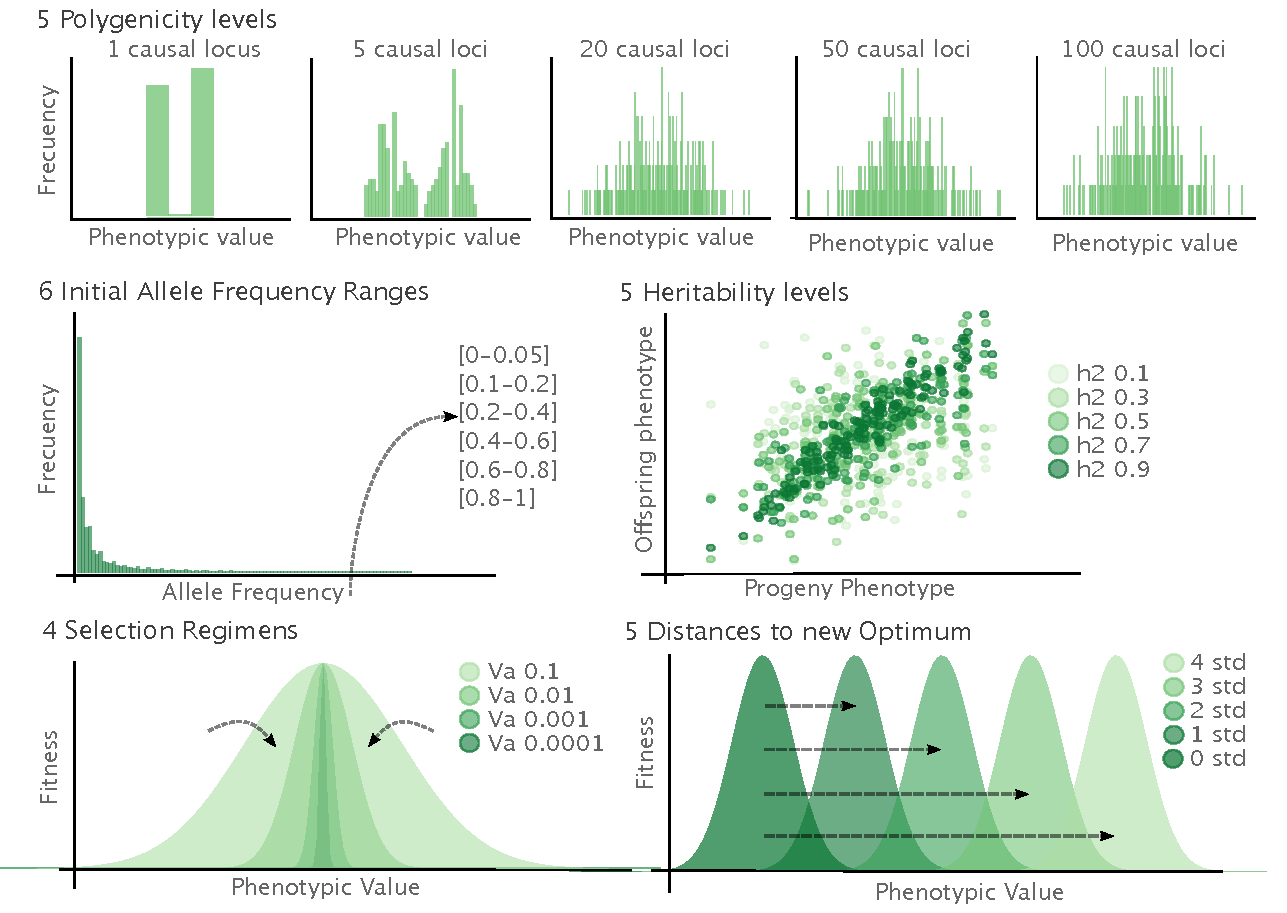
\includegraphics[width=1\textwidth]{figures/parameters.pdf}
    5\captionsetup{font=small} 
    \caption{Parameters used in the simulations. This figure outlines the comprehensive set of parameters used for the simulations, including the number of contributing loci or polygenicity [1, 5, 20, 50, 100, 200], the initial allele frequency ranges of the contributing loci[0-0.05, 0.1-0.2, 0.2-0.4, 0.4-0.6, 0.6-0.8, 0.8-1], the heritability levels [0.1, 0.3, 0.5, 0.7, 0.9], the selection strength modeled as fitness decay regimens [Va=1, 0.1, 0.01, 0.001], and the distance to the new phenotypic optimum [standard deviations from initial phenotypic mean= 0, 1, 2, 3, 4]}
    \label{fig:parameters}
\end{figure}

\subsubsection{Population density control}
For all simulations, we set a capacity charge of 900 individuals. The starting population size was always 2310 individuals, but after the first selection episode, and on every cycle, if the population reached a size larger than 900 individuals, we randomly subtracted individuals to keep it at 900. This is based on the observations of the real experiment, where the largest populations only reached a maximum of 900 individuals. 

\subsubsection{\textit{A. thaliana} biology}
Because one of our main focus was to tailor our simulations to the GrENE-net project, we decided to add some characters specific to \textit{Arabidopsis thaliana}, besides the founder populations' genetic diversity. Firstly, we used \textit{A. thaliana}'s mean recombination rate across the genome of $3 \times 10^{-6}$ (cite). Secondly, we simulated non-overlapping generations mimicking the plant annual cycle. Finally, we decided to use strict information about \textit{A. thaliana} reproductive strategies, simulating a 97\% selfing rate, 3\% out crossing rate (\citep{Platt2010-hy}), and a offspring size taken from $\sim Poisson(7.247)$,  based on an experimental average informed from common garden experiments (Exposito-Alonso lab, unpublished). 

\subsubsection{Tree sequence structure to simulate full genomes}

%The benchmarking of the software designed to detect adaptive loci would highly depend on the quality and realism of the genetic data coming from the simulated populations. With this in mind, 
Because we wanted to work with real genetic data to make our simulations highly realistic, we took advantage of the novel tree sequence structure and smooth SliM integration to simulate \textit{A. thaliana} genomes on its fullest \citep{Kelleher2018-jb, Haller2019-lm}. First, we converted the Variant Call Format (VCF) founder populations of 3,000,000 SNPs  into a tree sequence structure with the python module tsinfer \citep{Kelleher2019-ev}. Second, based on each simulation's genetic architecture we selected the loci contributing to the trait value. Thirdly, based on the principle that neutral mutations are just hitchhikers, we subtracted from the tree and separately saved all mutations not contributing to the trait. The resultant tree was lighter and fast to run on SLiM. Lastly, after each simulation finished, we overlaid the previously removed neutral mutations on the survival tree branches, obtaining as the final result the tree sequence with neutral and adaptive/non adaptive mutations on its fullest. 
\url{https://github.com/tskit-dev/pyslim}. 

\subsubsection{Reproducibility}
To ensure reproducibility and trackability of all analysis, we developed a snakemake pipeline \citep{Molder2021-ho}  starting with the initial VCF file from the founder populations and simulating all the parameters combinations. If desired, the pipeline could be rerun on its fullest. The code for the is available at \url{https://github.com/Tatianabellagio/slim_grenenet}.

\subsection{Readouts from population simulations}
Besides obtaining the full genomic dataset at the end of each simulation,  we extracted at each generation the population size, pseudo environment variables, individual genetic values, phenotypes and fitness. 

\subsection{Analyses from population simulation readouts}

\subsubsection{Statistical models to explain evolutionary outcomes of populations}

Using the population outcomes and the starting parameters of the simulation we can study the relationship among each of the parameters and the populations' survivorship. To do this, we run a Multiple Linear Regression (MLR) and multiple runs of Logistic Regressions (LR) with the Python module Statsmodels \citep{Seabold2010-ec}. 

\section{Results}

\subsection{Simulation parameters defining population mortality vs adaptation}
In order to understand the relevance of each parameter on the populations' ability to adapt, we ran a Multivariate Linear Regression (MLR) with all different parameters as regressors and populations' survivorship (0 or 1) at the 10\textsuperscript{th} generation as the predictor variable. In Fig. \ref{fig:glm_logisticreg} A, we report the slopes fitted for the MLR divided by the estimated error, i.e., their effect size or t-value for each parameter. This showed that, as expected, the distance to the moving environmental optimum had the strongest impact on the populations' survivorship (estimate = -2.39, t-value = -188.48, $p<1 \times 10^{-30}$), followed by the strength of selection as fitness decay (estimate =-1.95, t-value=-170.88,  $p<1 \times 10^{-30}$). Heritability followed, increasing the probability of survival (estimate = 0.65, t-value = 80.144, $p<1 \times 10^{-30}$). Surprisingly polygenicity showed a slight positive effect  (estimate =0.25, t-value=32.378,  $p=7.77 \times 10^{-3}$) and the frequency of the coding alleles in the initial population showed the smallest impact on the population's survivorship (estimate = -0.04, t-value=-5.33,  $p=7.66 \times 10^{-3}$).

Because we expected some of the parameters to have non-linear and context-dependent effects, we then conducted independent logistic regressions for fixed parameter combinations to marginally assess the effect and significance of a given parameter on survivorship (Fig. \ref{fig:glm_logisticreg} B). For this analysis, we obtained a distribution of t-values for each parameter, e.g., polygenicity, against a background of other parameter combinations, e.g., heritability-starting allele frequency-strength of selection-optimum distance. We only considered slopes with a p-value lower than 0.05 after Bonferroni correction. This analysis reconfirmed the MLR results for selection strength and distance to the new optimum and allowed us to question the effects of heritability, initial allele frequency, and polygenicity on the populations' probability of survivorship. These parameters showed a distribution of t-values and estimated coefficients ranging from positive to negative values.

\begin{figure}[h]
    \centering
    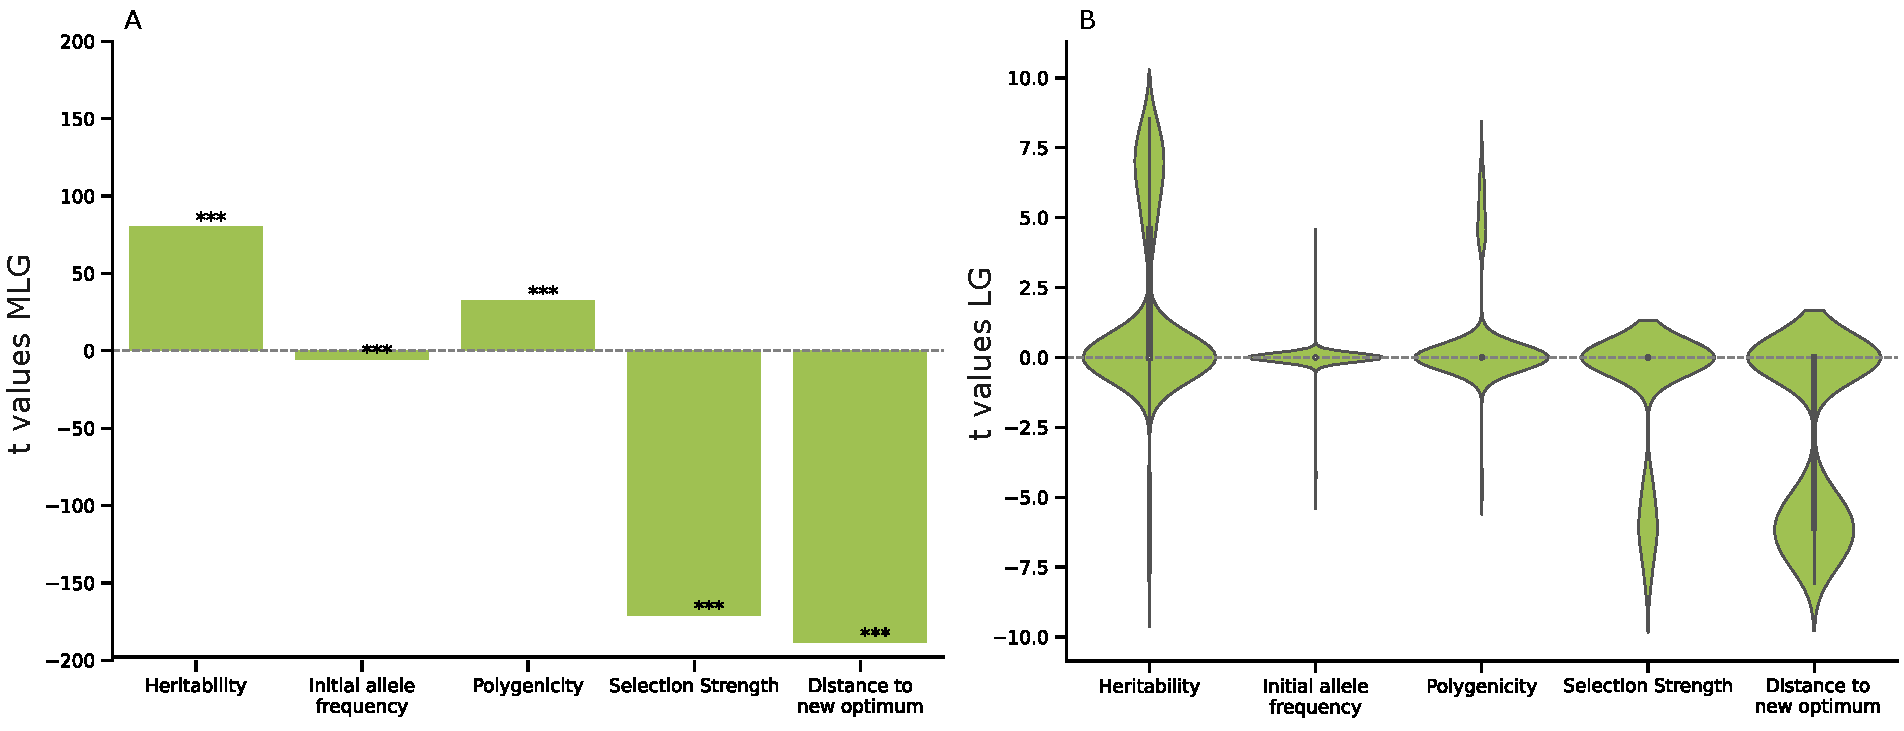
\includegraphics[width=1\textwidth]{figures/glm_logisticreg_newver.pdf}
    \caption{Impact of the simulation parameters on the populations' survival.  Panel \textbf{A} displays the outcomes of the Multivariate Linear Regression (MLR) with all parameters as predictors for binary survival. The bars indicates the MLR t-values, indicating the strength and direction of the relationship between each parameter and the population's adaptability. Asterisks denote levels of significance. Panel \textbf{B} shows the results obtained by running the
    Logistic Regressions (LR) for each parameter while holding all others constant. The violin plots represent the distribution of t-values obtained across all LR. Only parameters with p-values less than 0.05 after Bonferroni correction are shown.}
    \label{fig:glm_logisticreg}
\end{figure}


\subsection{Higher polygenicity allows populations to conquer extremer novel environments}
When fitness decay is not too strong to put populations at extinction risk, or the populations are close enough to the new optimum, polygenicity does not determine a population's survivorship probability (t-values close to 0 Fig. \ref{fig:poly_panel_figure} A, lower left corner). Nor does it when fitness decay is too steep or the new optimum is very far from the initial population, as most populations will inevitably perish regardless of genetic architecture (Fig. \ref{fig:poly_panel_figure} A, upper right corner).

At the 'extinction edges', defined as the intersection of selection strengths and distance to the new optimum where populations have at least 10\% but not more than 90\% survivorship rate at the 10\textsuperscript{th} generation (Fig. \ref{fig:poly_panel_figure} A and B, diagonal from upper left to lower right), we find a strikingly strong pattern where an increase in polygenicity has an overall positive effect on the populations' survivorship (Fig. \ref{fig:poly_panel_figure}  C, slope estimate = 0.27, t-value=56.23,  $p<1 \times 10^{-30}$). This aligns with population size measurements from Fig. \ref{fig:pop_size_poly_gen10}, where populations with higher polygenic traits are able to conquer environments of new optimum further away, compared with lower polygenic architectures in the 10\textsuperscript{th} generation.

Polygenicity seems to be beneficial mostly at further optima (directional selection) and not as strongly under stabilizing selection (Fig. \ref{fig:poly_panel_figure}, bottom row). We also observe that polygenicity tends to have a positive effect on survivorship only at higher heritability values (Fig. \ref{fig:poly_panel_figure}). Only in four cases do we observe a negative relationship between survivorship and increased polygenicity; these are isolated cases at very low allele frequencies and when the new optimum is far away (Slope estimates = -7.43, -1.601, -7.19, -0.81, t-values=-4.17 , -4.97, -4.44, -4.52,  all $p<1 \times 10^{-5}$). In these cases, we expect that rare phenotypes away from the original optimum but close to the new optimum caused by monogenic architectures may allow a rare  advantage.

\begin{figure}[H]
    \centering
    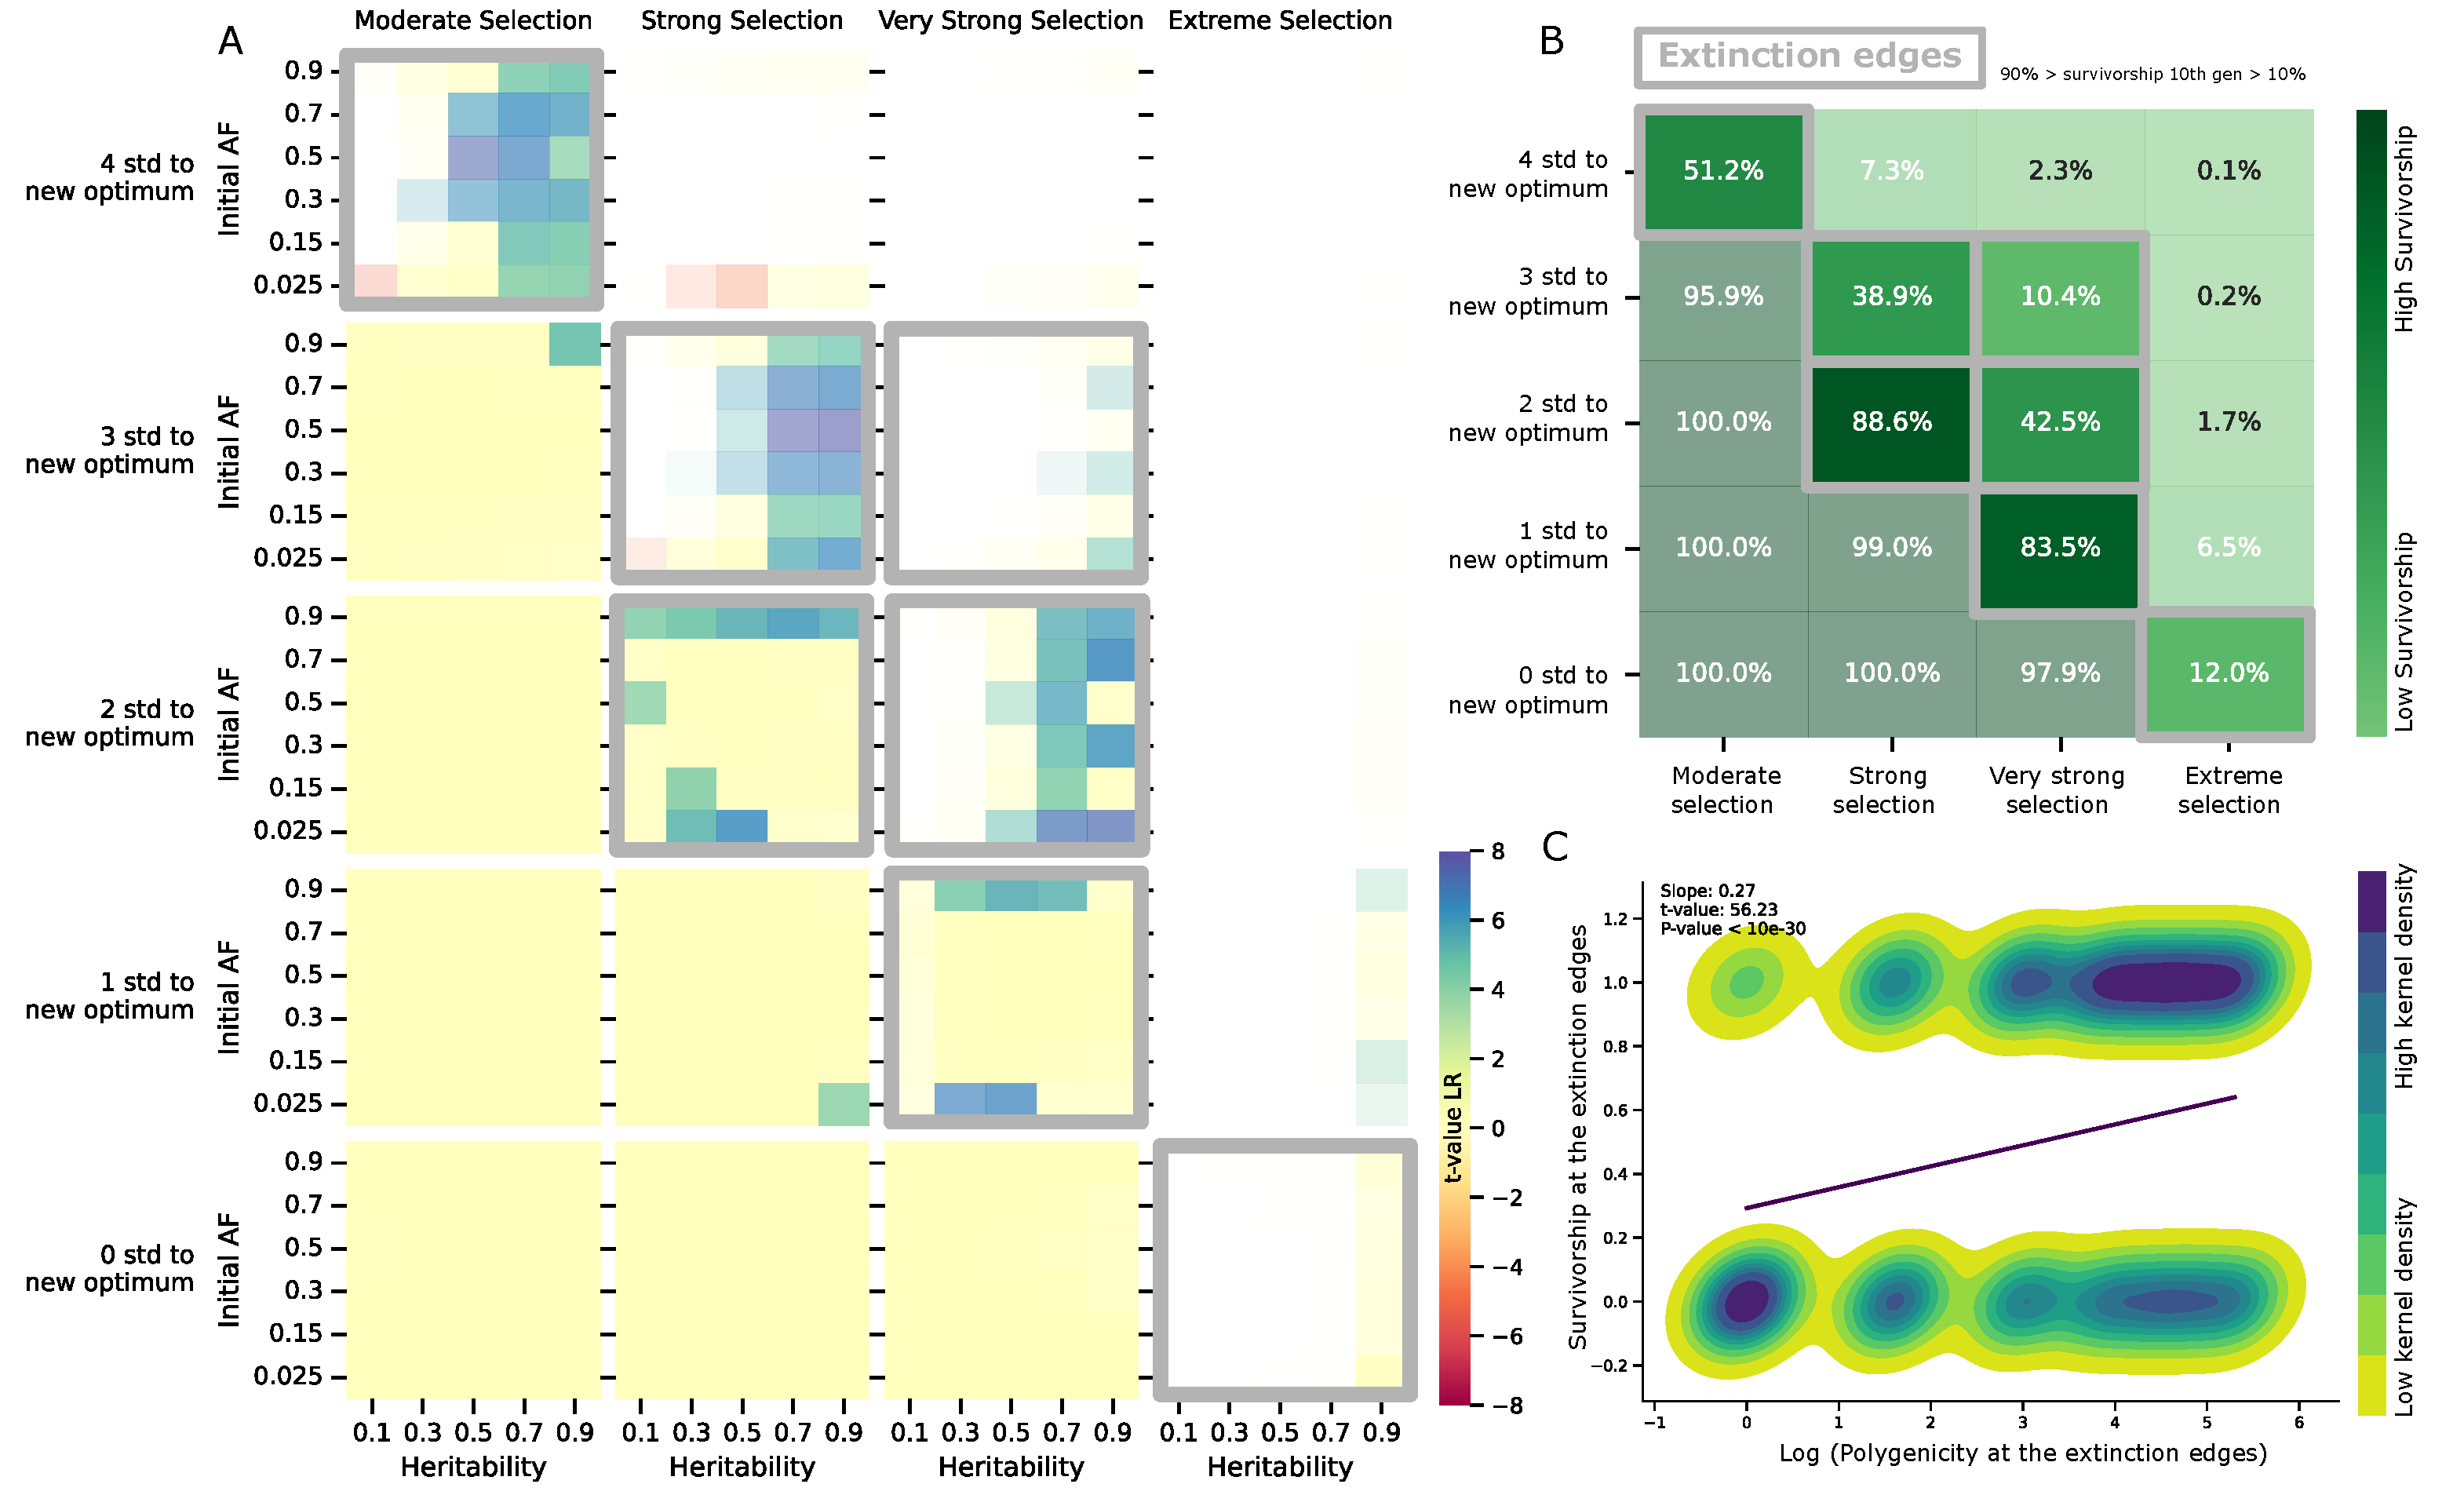
\includegraphics[width=1\textwidth]{figures/poly_survivalship_value_edges.pdf}
    \caption{Impact of polygenicity on populations' survival after the 10\textsuperscript{th} generation. Panel \textbf{A} illustrates the effect of the number of contributing alleles (polygenicity) on populations' survivorship through the fitted logistic regression slopes between polygenicity and survivorship. Each colored square represents one t-value value when all the remaining parameters are kept constant as indicated in the figure's legend (heritability, range of initial allele frequency, distance to new phenotypic optimum and selection strength), providing a comprehensive view of how polygenicity determines adaptation probability in the context of the other parameters. Furthermore,  the survival rates of populations are superimposed with varying degrees of transparency, visually emphasizing areas of lower (less transparency) or higher mortality (more transparency). Panel \textbf{B} showcase the 'extinction edges'. When taking into account the two most determining parameters on population's survivorship -distance to new phenotypic optimum and selection strength- the extinction edges are defined as the combination of these two parameters where population's survival rates are at least 10\%, but no more than 90\%. In panel \textbf{C}, the positive relationship between survival percentage and an increase in the log of polygenicity at the extinction edges is displayed (slope estimate = 0.27, t-value=56.23,  $p<1 \times 10^{-30}$)}
    \label{fig:poly_panel_figure}
\end{figure}

\begin{figure}[H]
    \centering
    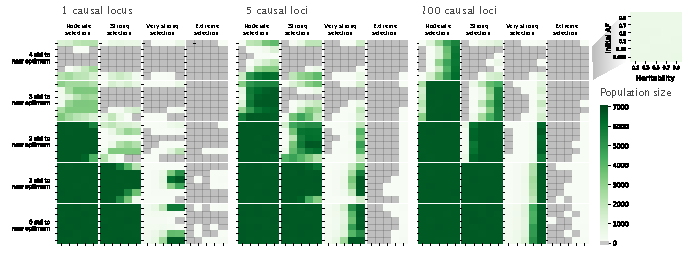
\includegraphics[width=1\textwidth]{figures/pop_size_GEN10.pdf}
    \caption{Populations sizes at generation 10 based on different genetic architectures, selection strength and distance to new optimum. Each color's square represents the average population size of the simulated replicates based on the given value for initial allele frequency, number of contributing loci, heritability, distance to new optimum, and selection strength at generation 10. When the square is marked in grey, all population replicates under the given conditions went extinct.}
    \label{fig:pop_size_poly_gen10}
\end{figure}

\subsection{High heritability does not consistently increase population's ability to adapt to changing environments}

In concordance with the results of high polygenicity being positive, high heritability is also  important to adapt at the extinction edges (Fig. \ref{fig:h2_panel_figure} A). Consistent with the observations in Fig. \ref{fig:glm_logisticreg}, heritability generally has a positive effect on a population's survivorship at the extinction edges (Fig. \ref{fig:h2_panel_figure} B, slope estimate = 2.59, t-value=79.51,  $p<1 \times 10^{-30}$).  

In concordance with what it is observed in Fig. \ref{fig:pop_size_poly_gen10}, higher heritability in polygenic architectures almost consistently conveys the population with a higher population size at further optima (Fig. \ref{fig:h2_panel_figure} B Polygenic architectures, slope estimate = 1.69, t-value=38.33,  $p<1 \times 10^{-30}$). However, the positive relationship between heritability and survival, weakens as the trait's polygenicity decreases. In scenarios involving traits with low polygenicity, the association between heritability and population survival weakens (slope estimate = 1.05, t-value=19.14,  $p<1 \times 10^{-30}$), and is almost zero for monogenic cases (slope estimate = 0.2, t-value=2.35,  $p=1.86 \times 10^{-2}$). Additionally, there are several instances where high heritability leads to lower survival. These instances occur under various initial allele frequencies and are specifically observed in low polygenic architectures (Fig. \ref{fig:h2_panel_figure}, slope estimates = -6.13, -7.33 , -0.59, -1.81, -1.44 , -0.93, -0.76, -0.63 , -1.16, t-values=-4.12, -4.39, -4.37265029, -5.53, -6.26, -6.15, -4.87, -4.61 , -5.15,  all $p<1 \times 10^{-5}$).

\begin{figure}[h]
    \centering
    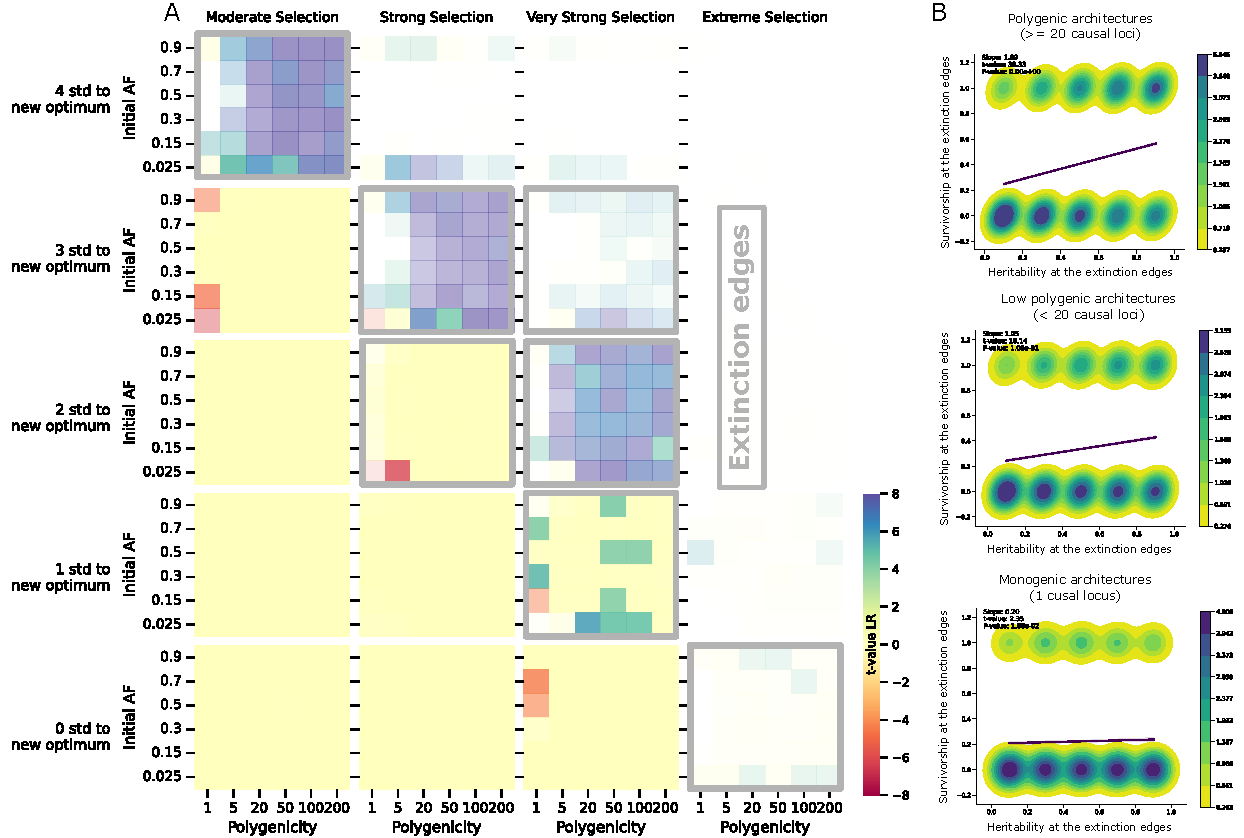
\includegraphics[width=1\textwidth]{figures/heristabilityvs_survivo_edges.pdf}
    \caption{Impact of heritability on populations' survival. Panel \textbf{A} illustrates the effect of heritability on populations' survival rates through the fitted logistic regression t-values between heritability and survivorship. Each colored square represents one t-values when all the  all the remaining parameters are kept constant as indicated in the figure's legend (polygenicity, range of initial allele frequency, distance to new phenotypic optimum and selection strength), providing a comprehensive view of how heritability determines adaptation probability in the context of the other parameters. Furthermore,  the survival rates of populations are superimposed with varying degrees of transparency, visually emphasizing areas of lower (less transparency) or higher mortality (more transparency). In panel \textbf{B} the fitted lines for the relationship between population's survival and heritability at the extinction edges are reported at three different polygenicity levels, showcasing that the relevance of heritability is dependent on the polygenicity level. Polygenic architectures (slope estimate = 1.69, t-value=38.33,  $p<1 \times 10^{-30}$), low polygenic architectures (slope estimate = 1.05, t-value=19.14,  $p<1 \times 10^{-30}$ ) and monogenic architectures (slope estimate = 0.2, t-value=2.35,  $p=1.86 \times 10^{-2}$)}
    \label{fig:h2_panel_figure}
\end{figure}

\subsection{Genetic architecture is a key factor defining mean fitness and fitness variance at the extinction edges}

Based on the context-dependent results of the connection between genetic architectures and population survival, we explored further the evolutionary dynamics based on genetic architecture at the extinction edges. We zoomed into the simulations with selection strength of $Vs=0.01$  and 2 standard deviations from the optimum, as this is the parameter space that led to significant and varying correlations of genetic architecture with population's survival (Fig. \ref{fig:pop_size_poly_gen10, fig:poly_panel_figure}). 

At high heritability levels (Heritability = 0.9), we noted that populations with higher polygenic architectures attained greater mean fitness and fitness variance than those with lower polygenic traits (Fig. \ref{fig:mean_fitness_acrossgen}, Fig. \ref{fig:var_fitness_across_gen}). Specifically, the mean fitness variance across initial allele frequencies at the 10\textsuperscript{th} generation was $0.02$ for 1 causal locus, $8 \times 10^{-2}$  for 5 causal loci, and $0.09$  for $\geq 20$ causal loci. Correspondingly, the mean of fitness means was $0.1$ for 1 causal locus, $0.47$  for 5 causal loci, and between $0.64- 0.65$  for $\geq 20$ causal loci. Notably, the variance across replicated simulations in mean fitness, $\bar{w}$ and fitness variances, $V_w$ , across initial allele frequencies exhibits a striking contrast when comparing low and high polygenic architectures at these high heritability levels in the final generation. For instance, the variance in $V_w$  was $1.445 \times 10^{-3}$ for 1 causal locus, $1.149 \times 10^{-3}$ for 5 causal loci, and between $1.7-4.1 \times 10^{-5}$ for $\geq 20$ causal loci, while the variance of $\bar{w}$  was $3.6 \times 10^{-2}$ for 1 causal locus, $5.8 \times 10^{-2}$ for 5 causal loci, and between $3 \times 10^{-3} - 2.8 \times 10^{-4}$ for $\geq 20$ causal loci. This pattern underscores the fact that low polygenic architectures lead to more stochastic simulations, where the idiosyncrasy created by only one or few alleles controlling one trait leads to more variable fitness means and variances across population simulations, whereas high polygenic architectures have fitness means and variances that are more consistent across population simulations that are less affected by the randomness of the initial conditions.

Intriguingly, low heritability (Heritability = 0.1), produced more robust starting fitness mean and variances, than high heritability cases (Fig. \ref{fig:mean_fitness_acrossgen}, Fig. \ref{fig:var_fitness_across_gen}). The mean fitness variances were $3.5 \times 10^{-2}$ for 1 causal locus, $6.6 \times 10^{-2}$ for 5 causal loci, and between $6.6-8.2 \times 10^{-2}$ for $\geq 20$ causal loci, while the mean of fitness means were $6.9 \times 10^{-2}$ for 1 causal locus, $1.35.8 \times 10^{-1}$ for 5 causal loci, and between $1.4- 1.5 \times 10^{-1}$ for $\geq 20$ causal loci. We believe these results explain  the observations in Fig. \ref{fig:h2_panel_figure}, where low heritability positively correlated with survival at low polygenic architectures. 

\begin{figure}[H]
    \centering
    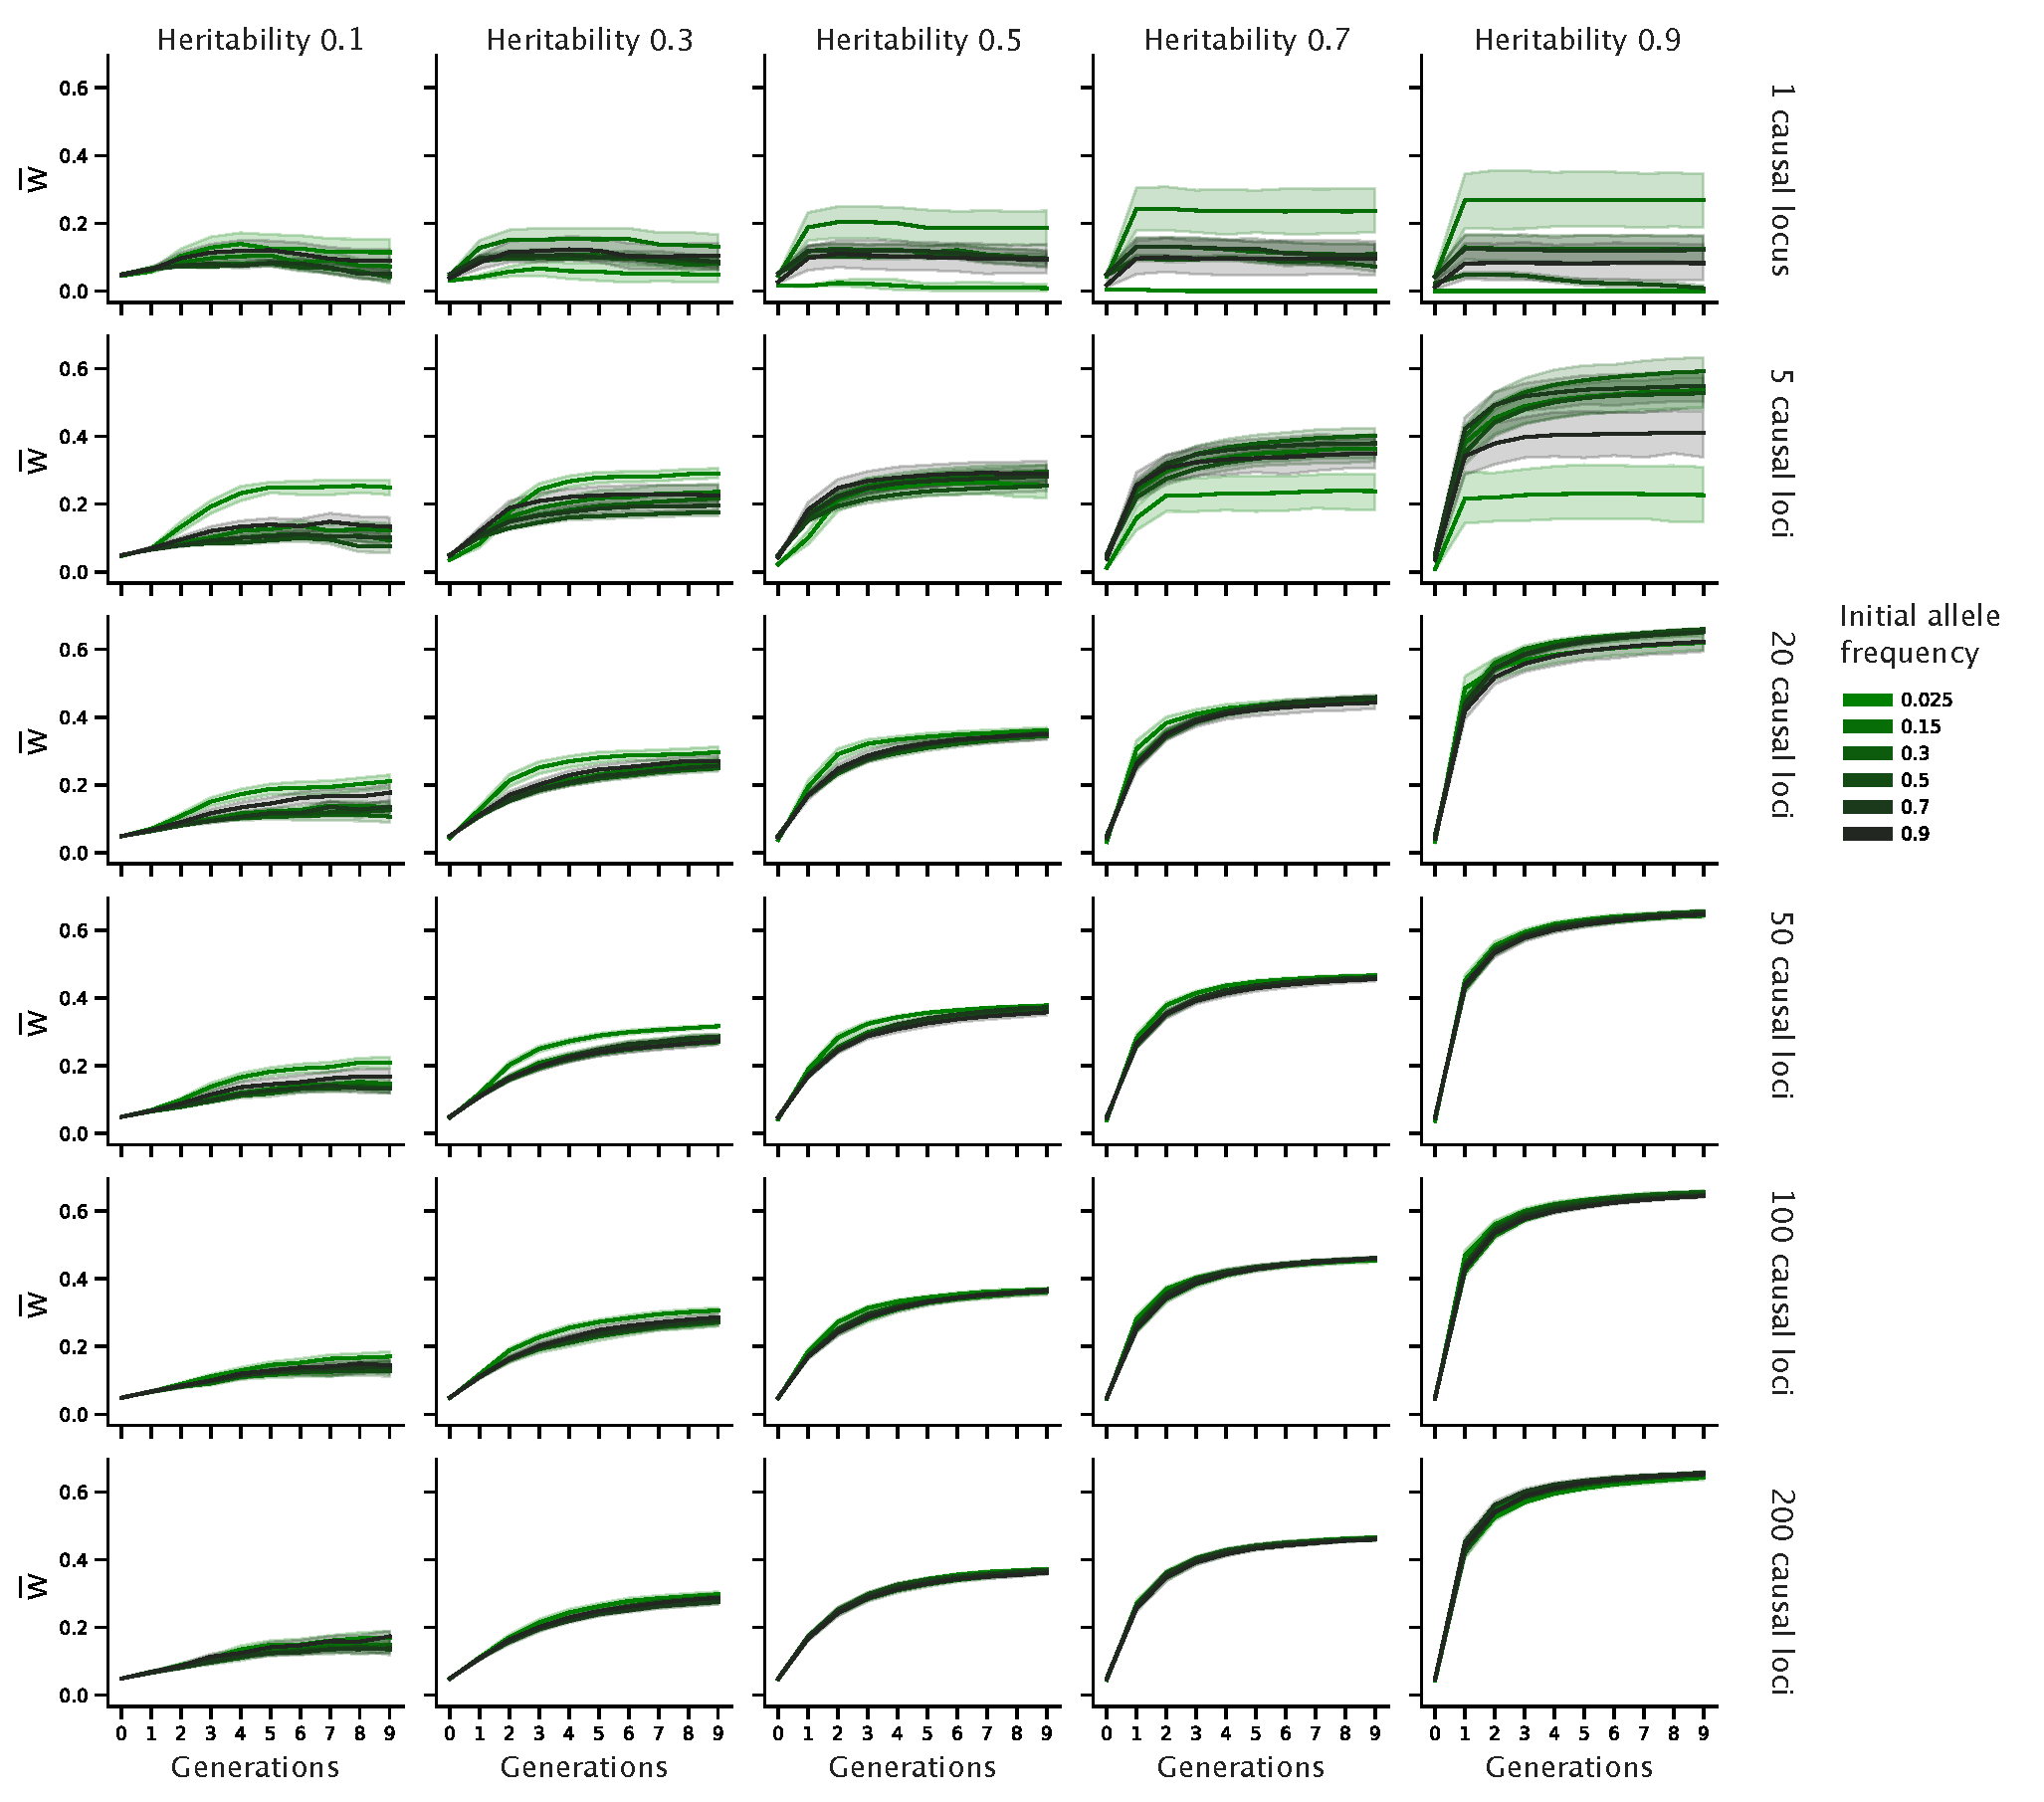
\includegraphics[width=1\textwidth]{figures/mean_fitness_acrossgen.pdf}
    \caption{Evolution of mean fitness at the extinction edges based on genetic architecture. Changes in mean fitness across generation for different initial allele frequencies, polygenicity, and heritabilty levels. These results correspond to simulations with a fixed selection strength of Vs = 0.01 and whose new optimum was situated 2 standard deviations from the initial population phenotypic mean.}
    \label{fig:mean_fitness_acrossgen}
\end{figure}

\begin{figure}[H]
    \centering
    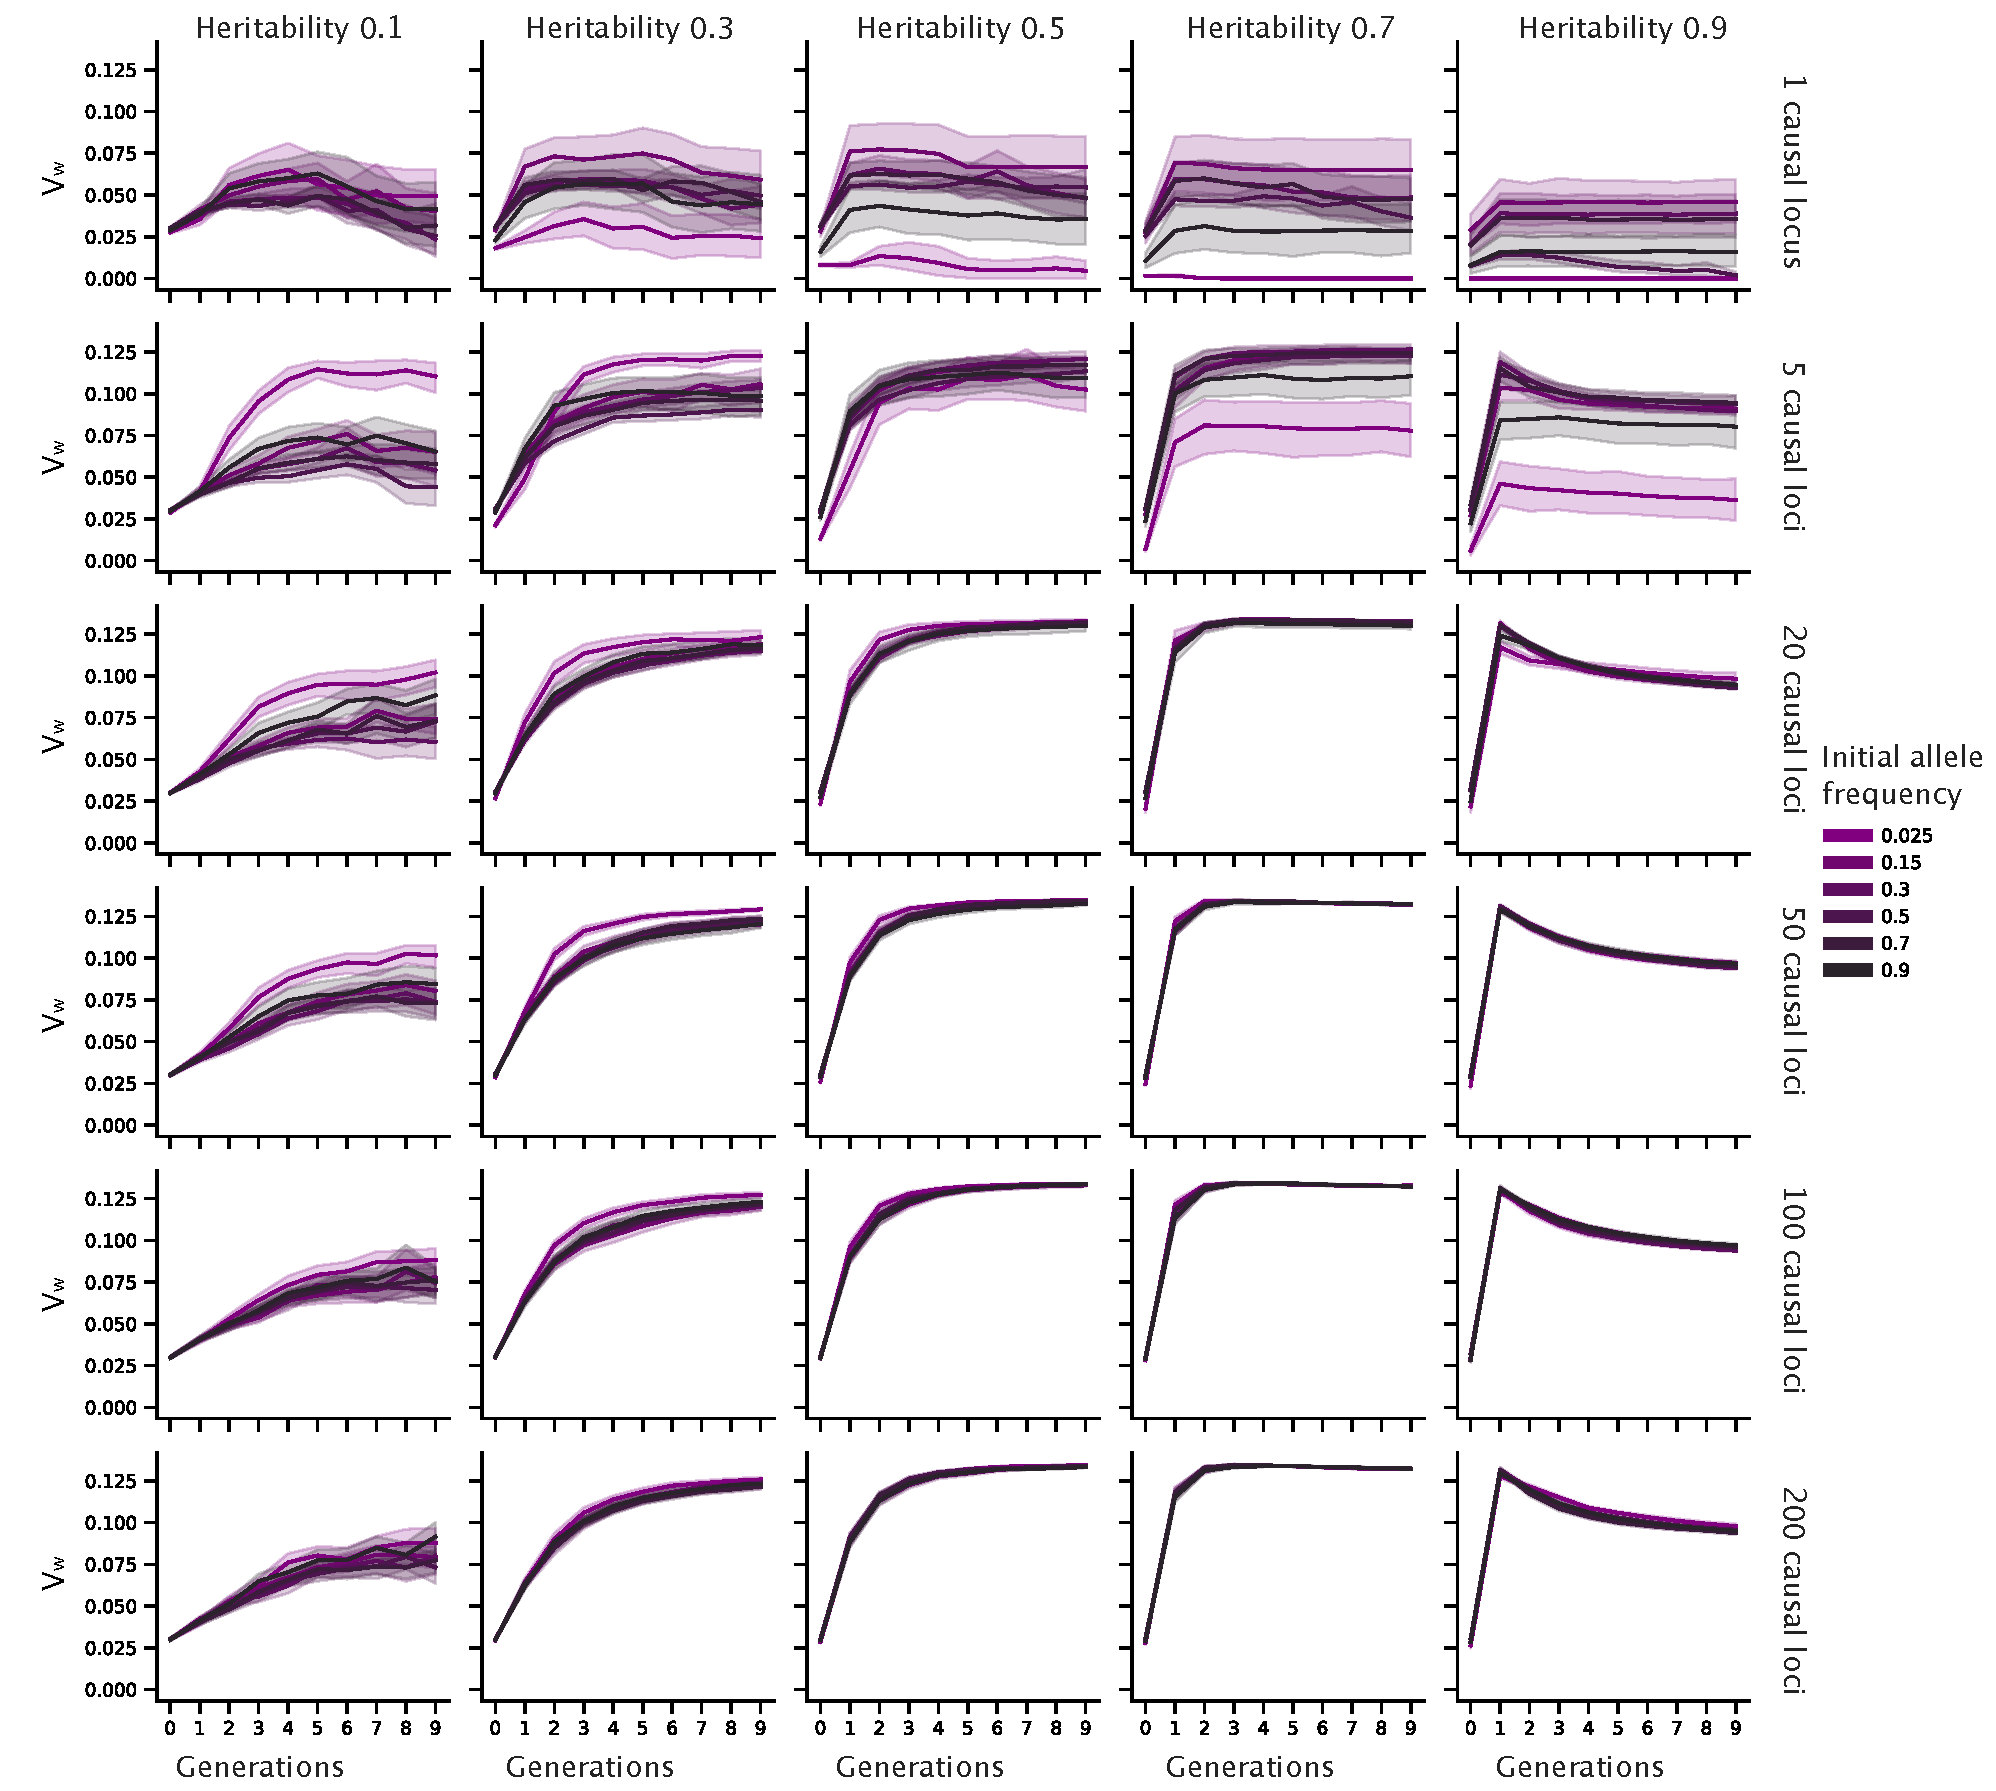
\includegraphics[width=1\textwidth]{figures/var_fitness_across_gen.pdf}
    \caption{Evolution of fitness variance at the extinction edges based on genetic architecture. Changes in fitness variance across generation for different initial allele frequencies, polygenicity and heritabilty levels. These results correspond to simulations with a fixed selection strength of Vs = 0.01 and whose new optimum was situated 2 standard deviations from the initial population phenotypic mean.}
    \label{fig:var_fitness_across_gen}
\end{figure}

\section{Discussion}

With environments changing faster than ever, understanding the evolutionary dynamics of rapid adaptation has become of utmost interests. Application of this knowledge range from invasive species management (Lee 2002; Lee and Gelembiuk 2008), applied evolutionary rescue for species at extinction risk, or even understanding concerning medical issues such as the emergence of novel infectious diseases where genetic adaptation to a novel host is required (Holt and Hochberg 2002; Antia et al. 2003)

Rapid adaptation has been widely documented as shown in the examples listed in the introduction. Nonetheless, this does not mean that it can always occur. The mentioned examples highlight the \textbf{potential}, in principle, for rapid adaptation to overcome environmental changes. However,  the large declines of populations across species could be indicative that adaptation to rapid environmental changes is not the rule (cite extinction list IPBES). Decades ago, theoretical work with simplified population genetic models concluded that regardless of the genetic model, even populations with the necessary genetic variation to adapt, may still often fail to do so in novel environments  \citep{Gomulkiewicz1995-sj}. We therefore need to better understand when evolutionary outcomes will fail, and for that we need better understanding on key evolutionary and population parameters in realistic simulations and experiments. For example, it is now widely regarded that the  probability  of  a population  survival  increases  with  both  population  size  and  the number of exchangeable loci (diversity) (\citep{Newman1997-tx, Markert2010-wc, Nabutanyi2022-jb}). Perhaps by identifying measurable parameters describing the genetics of a species, we may be able to improve practical management decisions for species conservation. 

\subsection{Why do polygenic traits show lower extinction rates and allow populations to survive in extreme environments?}

In our realistic simulations we showed that increased trait polygenicity has a positive effect on populations' survivorship probability at the extinction edges (Fig. \ref{fig:poly_panel_figure}). That is, this architecture allow populations to adapt in environments further away from the original optimum (Fig. \ref{fig:pop_size_poly_gen10}). We observed that this could be a result of this architecture consistently allowing populations achieving a high mean and fitness variance after the short period of 10 generations (Fig. \ref{fig:mean_fitness_acrossgen},  Fig. \ref{fig:var_fitness_across_gen}).

Previous literature on the relationship between rapid evolutionary outcomes and genetic architecture is inconclusive. Some foundational work on the topic by Gomulkiewicz \& Holt examined a quantitative-genetic model and a one-locus model, obtaining similar results in terms of evolutionary outcomes \citep{Gomulkiewicz1995-sj}. Orr and Unckless later highlighted evidence favoring polygenic architectures, arguing that it would be difficult for a single locus to adapt to rapid environmental change compared to multiple loci, a concept now referred to as genetic redundancy \citep{Laruson2020-kd}. Gomulkiewicz, in later theoretical work, however, showed analytically that increasing the number of loci contributing to a trait can decrease the speed of adaptation and prevent evolutionary rescue \citep{Gomulkiewicz2010-wr}.

The contrasting results obtained by Gomulkiewicz et al. and our study are based on the foundational assumptions of their study and ours. They used an additive model of mean Malthusian fitness of a population at time $t$
\[
m_t = \sum_{i=1}^{n} \left( p_{t,i}^2 m_{AA,i} + 2p_{t,i} q_{t,i} m_{Aa,i} + q_{t,i}^2 m_{aa,i} \right)
\]
where  
$n = \text{Number of loci}$, $p_{t,i} = \text{Frequency of allele A at locus } i \text{ at time } t$, 
$q_{t,i} = \text{Frequency of allele a at locus } i \text{ at time } t$, $m_{AA,i} = \text{Fitness of the AA genotype at locus } i$,
$m_{Aa,i} = \text{Fitness of the Aa genotype at locus } i$,
$m_{aa,i} = \text{Fitness of the aa genotype at locus } i $. They define $A$ as the advantageous allele at the new environment, and hence selection acts on the other two genotypes, so $m_{AA,i} = \frac{r_{\text{max}}}{n}$, $\text{ } m_{Aa,i} = \frac{r_{\text{max}}}{n - \frac{s_i}{2}} $, and $m_{aa,i} = \frac{r_{\text{max}}}{n - s_i} $
Where $r_{\text{max}}$ represent the maximum population growth and $s$ the selection coefficient. This equation encapsulates the assumption that initial fitness mean <<<and variance>>> is constant across architectures. From this initial equation, It's evident from this initial equation that there is an inverse relationship between the number of loci involved in the adaptation and the population growth rate, as larger $n$ weakens the selection at each locus. 

The reverse assumption, where Malthusiam fitness is not scaled by the number of loci: $m_{AA,i} = r_{\text{max}}}$ etcetera, shows clearly the opposite. When we instead of assuming mean fitness is constant, but rather selection per loci is constant, is easy to show that fitness will grow linearly with the number of adaptive loci. This assumption is also problematic.

In contrast, the model underlying our realistic simulations does not assume initial constant mean and fitness variance across architectures, instead we scale the adaptive trait of our population to have the same mean and variance across architectures. This assumption is achieved by standardizing all phenotypes to mean 0 and variance 1, in consequence, different architectures will reach the same distribution of phenotypes for fair comparison. Consequently, we assume that higher polygenic traits will have smaller per locus $V_a(z)$, by also diluting the total $V_a$ into the number of contributing loci. Nevertheless, as shown in Fig. \ref{fig:initial_pop_meanandvar_fitvar} A, when heritability is high, we observe the initial fitness mean $\bar{w}$ and variance $V(w)$ is highly dependent on the genetic architecture and can already notice higher fitness variance at that higher polygenic architectures have overall higher mean fitness values, despite the adaptive phenotype distributions across architectures are equal. This result alone might be enough to explain the higher extinction rates of lower polygenic architectures based on Fisher's fundamental theorem of adaptation where the additive genetic variance in fitness ($Va(w)$) determines the rate of adaptation over generations (Fisher, 1930). Consistently with our results, the mean  $V(w)$ across simulations of high polygenic architectures is higher than monogenic architectures (Fig. \ref{fig:initial_pop_meanandvar_fitvar}). This support the trajectory that these populations with high $V(w)$  reach survival in the last generation studied in Fig. \ref{fig:mean_fitness_acrossgen} and Fig. \ref{fig:var_fitness_across_gen}. Again, this supports the notion that the distribution of fitness $V(w)$  is highly dependent on the genetic architecture despite starting phenotype frequencies remaining the same, a pattern not accounted for in previous theoretical and simulation work (CITE MULTIPLE). Furthermore, previous studies have not explored the joint important parameter of varying heritability levels and finite population sizes or other realistic population parameters.   

The explanation for why low polygenic architectures, already at the simulation onset, show lower mean fitness variance and an increase in the variance of fitness variance requires further investigation. Our initial hypotheses are related to the nature of low polygenic traits, where the number of possible phenotypes is scarcer and highly dependent on the initial allele frequency of the contributing loci. This is supported by the fact that low polygenic architectures do not always have lower initial fitness variance, but the phenotypic outcome is heavily influenced by initial allele frequencies, leading to stochastic distributions and highly variable in $V(w$ (fig:initial_pop_meanandvar_fitvar). (add suplemental showing fitness variance in initial populations with varying initial alllele freq).

Furthermore, our results are in concordance with more recent work by Kardos \& Luikart \citep{Kardos2021-jd}. In their study, they used simulations to develop more realistic scenarios relevant for conservation biology, and demonstrated that population extinction is less likely in models with polygenic architectures compared with models with few large-effect loci. The authors argue that this is due to low-polygenic traits having lower short-term evolutionary potential (potential change in phenotype across generations).

\begin{figure}[H]
    \centering
    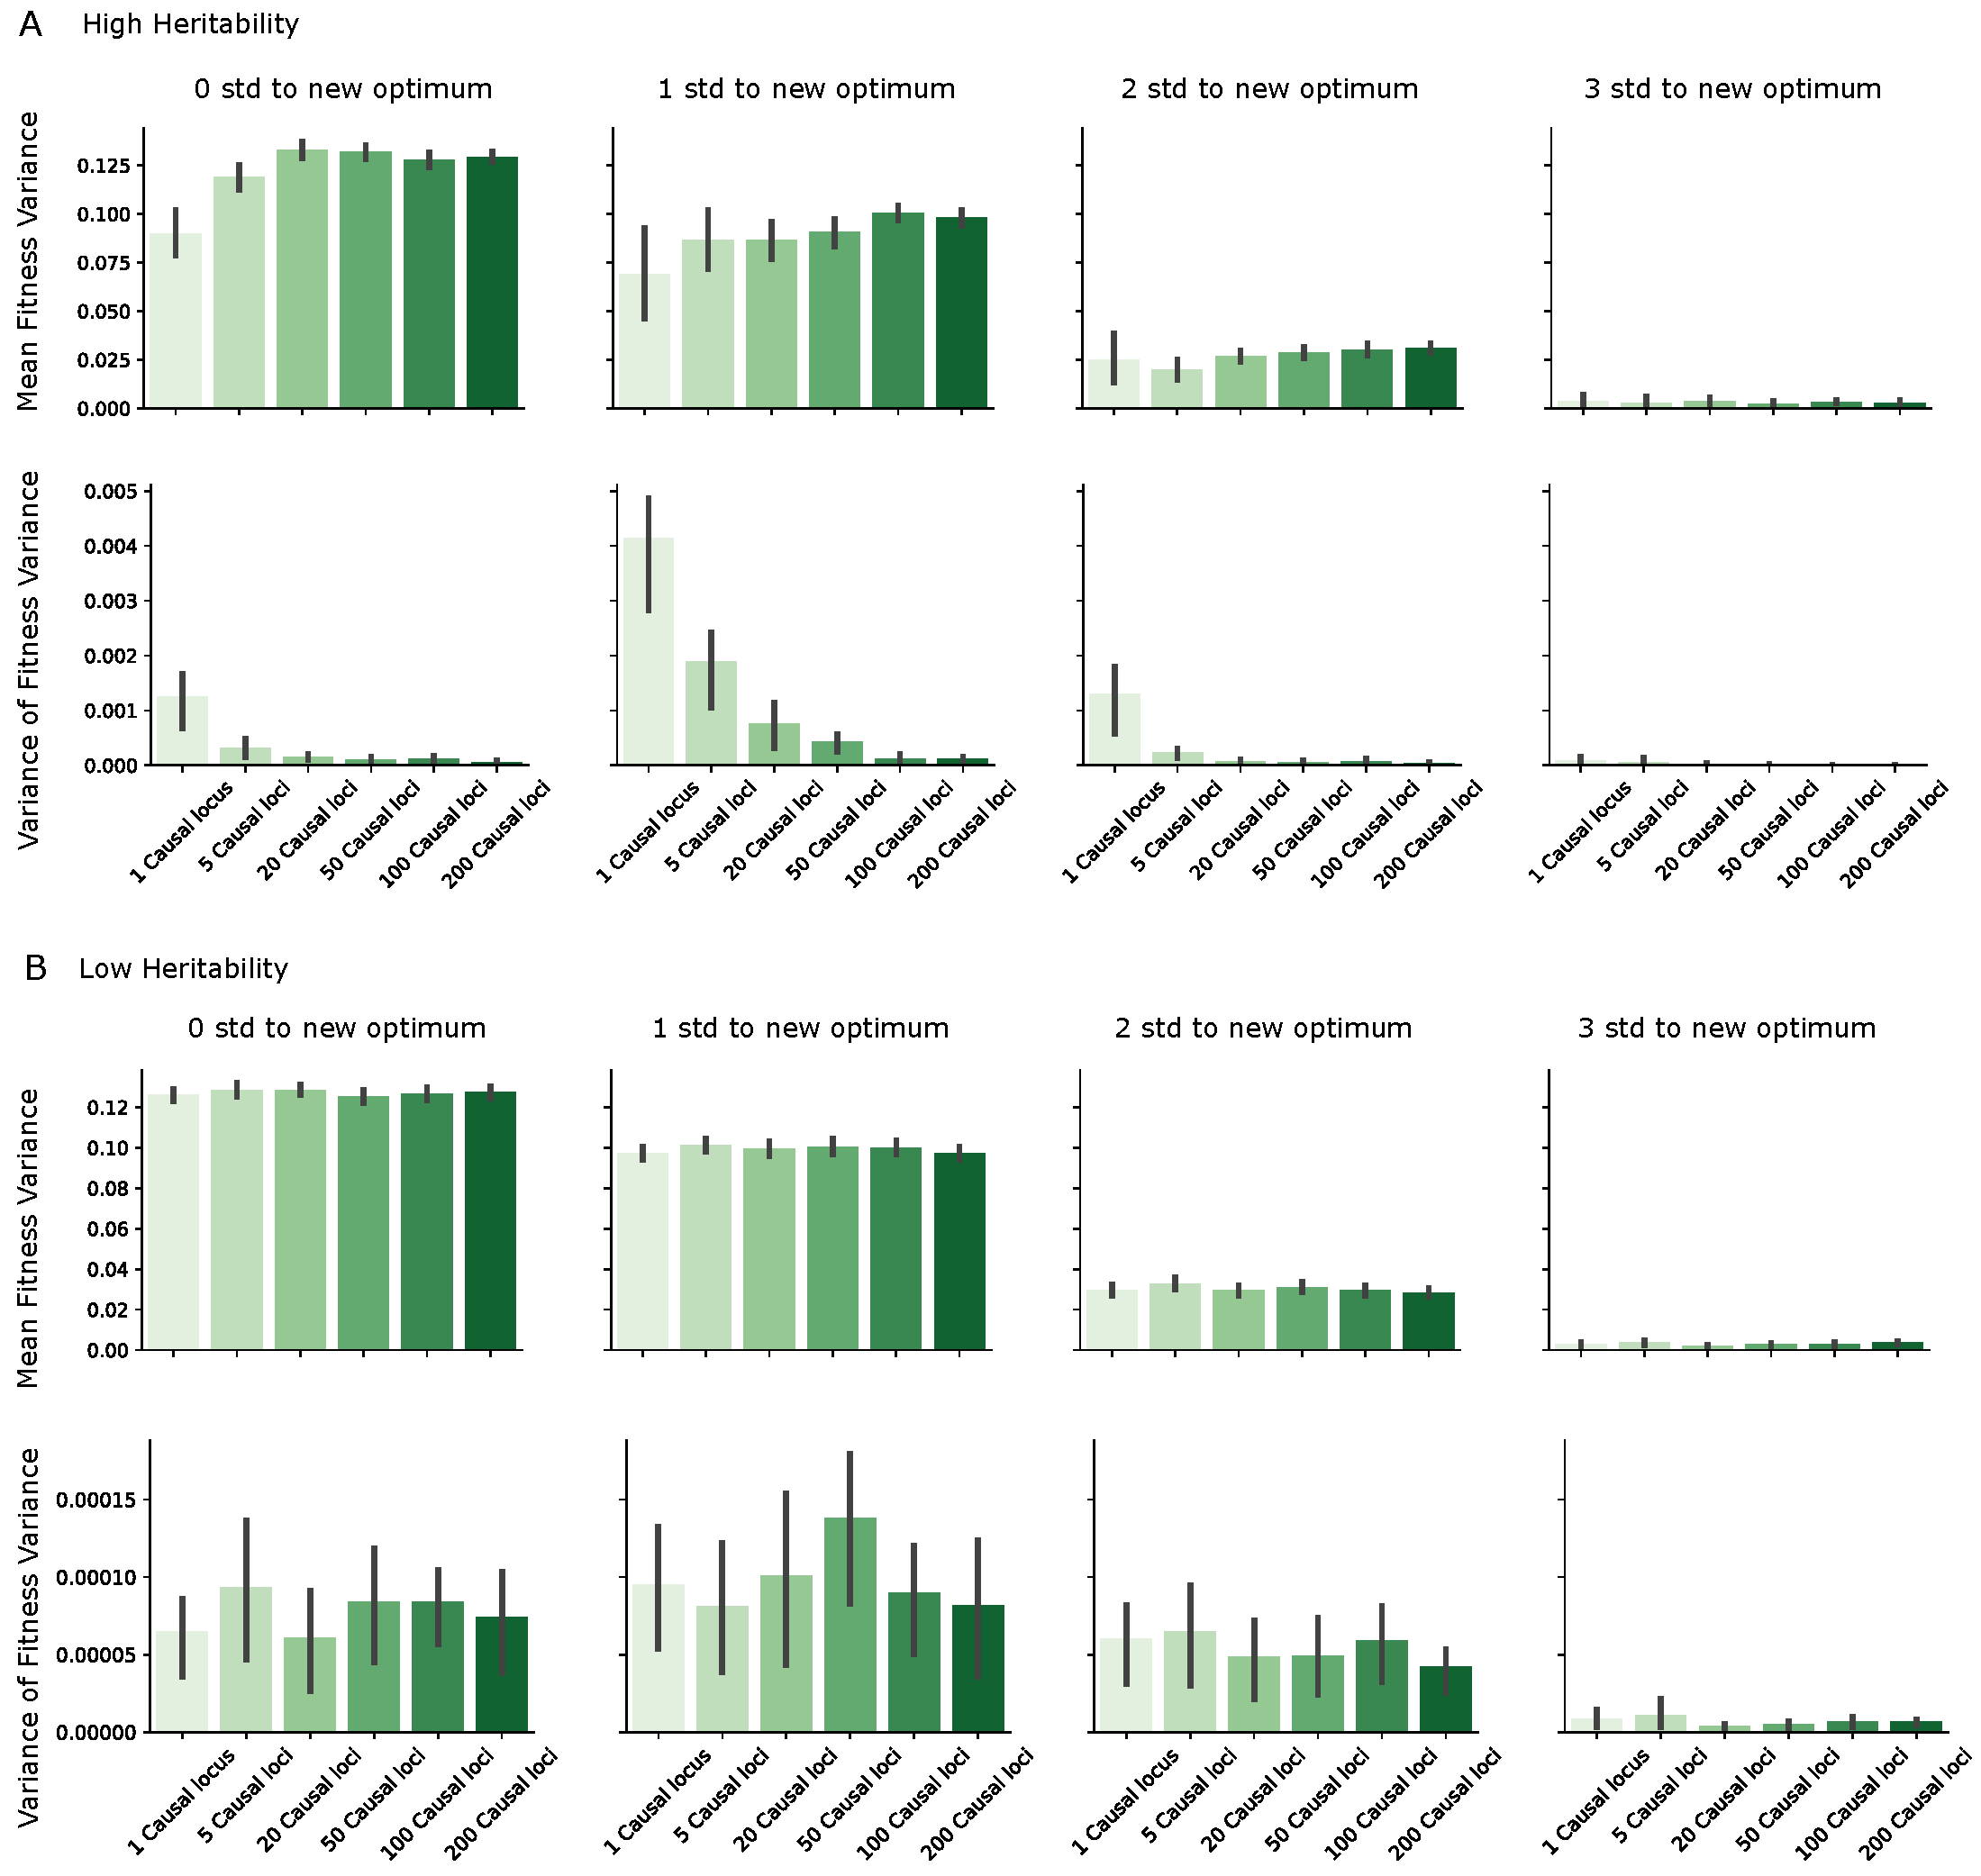
\includegraphics[width=1\textwidth]{figures/mean_var_of_fitness_var_ipop_sel0.1.pdf}
    \caption{Mean fitness variance and variance of fitness variance of initial populations across genetic architectures and distance to new optimum values at high and low heritability levels and strong selection. The mean fitness variance and the variance of the fitness variance for each level of polygenicity was calculated across all initial allele frequencies for the contributing loci and keeping constant a high heritability level of 0.9 and a regimen of strong selection (Vs = 0.1).}
    \label{fig:initial_pop_meanandvar_fitvar}
\end{figure}

\subsection{The Paradox of Heritability in Low Complexity Traits}

Contrary to intuition, our results showed that high heritability does not necessarily enhance survival in low-complexity genetic architectures in certain extreme environments. Even more strikingly, we found a negative relationship between increased heritability and population survival in some areas (Fig. \ref{fig:h2_panel_figure}). Interestingly, the pattern described in the section above is completely masked in initial populations with low heritability levels. Low and high polygenic architectures show similar values of mean fitness variance, and low polygenic architectures do not show higher variance of fitness variance either (Fig. \ref{fig:initial_pop_meanandvar_fitvar} B). Low heritability seems to introduce a 'buffering' effect, smoothing the phenotypic distribution and consequently fitness, while high heritability and low polygenicity led to strongly discrete phenotypes. 

Because our simulations were designed to be highly realistic and to match a real-world evolutionary experiment (GrENE-net) with \textit{Arabidopsis thaliana}, there could be concerns that our results are influenced by specific genetic characteristics of this species. This would include, high-linkage levels and a notable lack of homozygosity in the populations, which are indicative of alleles not being in Hardy-Weinberg equilibrium. Therefore, we conducted a set of additional simulations under the Wright-Fisher model (i.e. without any realistic and  \textit{Arabidopsis thaliana} specifications). These simpler, organism-agnostic simulations (not shown) supported these findings. 

\subsection{Polygenicity is not intrinsically better}

As Lande stated in 1983, adaptation through polygenic or monogenic traits is equally feasible \citep{Lande1983-kz}, and we concur, under the assumption that different architectures would lead to the same mean and variance fitness. However, under realistic simulations, we show that higher polygenic architecture will have overall distributions of fitness values with higher means and lower variances across initial allele frequencies of contributing loci. 

%will cover the phenotypic space in a more continuous and consistent manner, enhancing their odds to adaptation to further optima. 

We would like to highlight the fact that our results are true under the assumption that different genetic architectures can reach the same distribution of phenotypes, due to an inverse relationship between the number of contributing loci and Va at each locus. Furthermore our conclusions are drawn in the context of rapid adaptation solely based on standing variation. This is quite important, since an scenario in which the new optimum value is out of range and standing genetic variation is not enough to reach it, our observations might not prevail. 


\section{Conclusion}
We conclude that, if the population possesses the genetic diversity to adapt to the new imposed environmental optimum, polygenic architectures show lower extinction rates and are better suited to adapt and survive in environments with further values from original optimum due to their higher and more consistent overall mean fitness variance. Furthermore, while heritability is highly beneficial at higher polygenic architectures, we had the conterintuitive finding that certain extreme environments and low polygenic architectures would have lower probability of survival with highly heritable traits. We conclude low polygenic architectures show higher extinction rates across simulation replicates, as their fitness distribution is highly dependent on the initial allele frequency of contributing loci making them generally more susceptible to an extinction event. 

\bibliography{paperpile,extra}

\end{document}
